\chapter{Results and Discussion}

\section{Introduction}
This chapter presents the practical outcomes, implementation strategies, and key discussion points of the 2D-to-3D Image Conversion project. The pipeline consists of four major operational phases: Augmented Reality (AR)-based image acquisition, neural network-driven depth estimation, point cloud back-projection, and geometric surface reconstruction via the rolling ball algorithm. The following sections provide an in-depth analysis of each module's implementation and performance on a mobile edge device.

\section{ARCore-Based Data Acquisition and Image Capture}
The initial and most crucial step of the pipeline is the acquisition of high-quality, geometrically contextualized images. This was implemented using Google's ARCore framework integrated into the Flutter application.

\subsection{Spatial Anchoring and Tracking}
Instead of relying on a simple smartphone camera capture, the application initializes an AR session. This allows the system to perceive the physical environment while tracking feature points and planar surfaces. The user is prompted to place a virtual \textbf{Anchor} in the real world. This anchor acts as the absolute origin $(0,0,0)$ for the coordinate system of that specific scanning session. By localizing the capture around this anchor, the system achieves a grounded reference frame.

\subsection{Camera Position and Angle of Capture}
When the user triggers the capture mechanism, the system records not only RGB pixel data but also spatial metadata. The exact \textbf{camera position and orientation} (6 Degrees of Freedom - 6DoF) are recorded as a $4 \times 4$ relative pose matrix representing the camera's spatial relationship to the placed anchor. This specific angle of capture is vital; it ensures that, if the system is scaled to support multi-view stereo in the future, the transformation constraints between different viewing angles are preserved. To prevent spatial distortion during the neural network inference stage, the capture module enforces a strict 1:1 (square) aspect ratio crop, guaranteeing that the true proportions of the localized object are preserved.

\begin{figure}[H]
    \centering
    \makebox[\textwidth][c]{%
        \begin{minipage}[t]{0.53\textwidth}
            \centering
            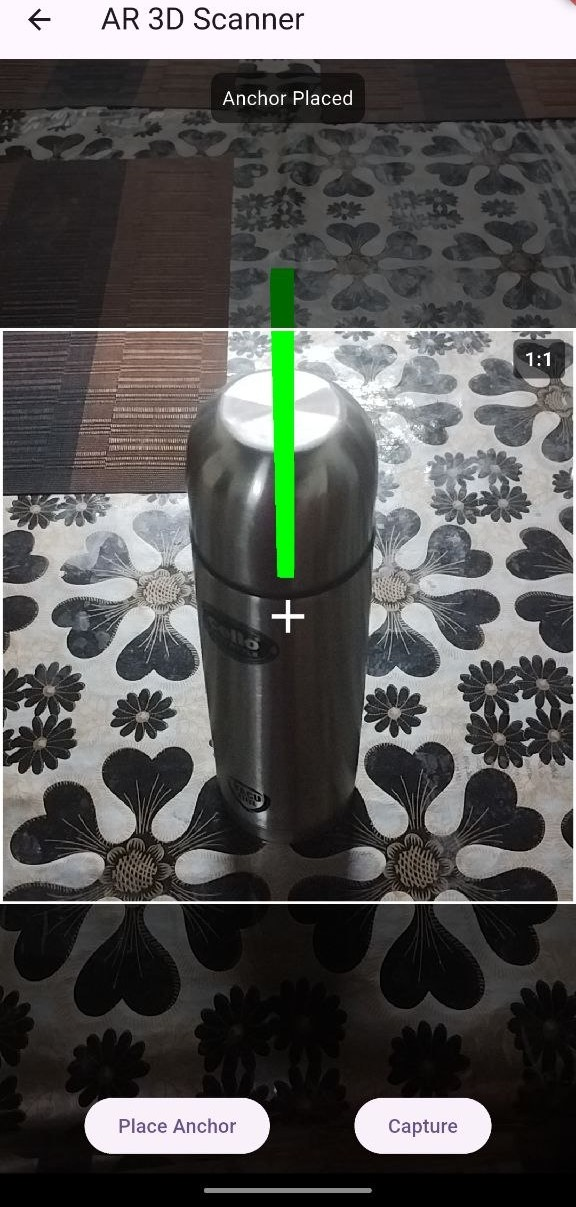
\includegraphics[width=\linewidth]{Images/capture1.jpg}
        \end{minipage}\hspace{0.04\textwidth}%
        \begin{minipage}[t]{0.53\textwidth}
            \centering
            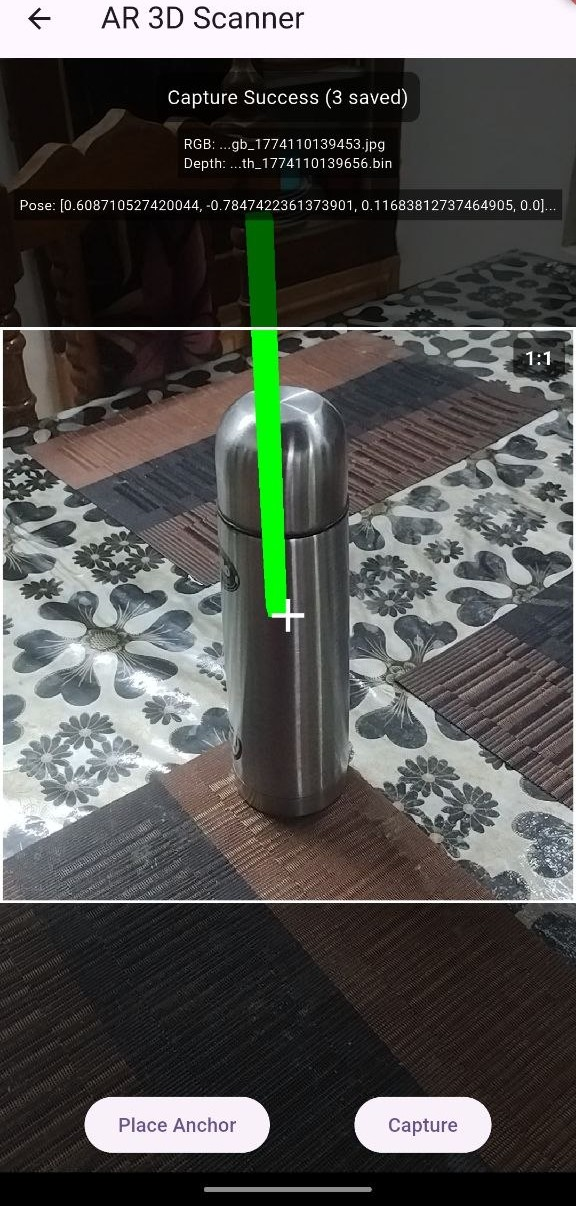
\includegraphics[width=\linewidth]{Images/capture2.jpg}
        \end{minipage}%
    }
    \vspace{10pt}
    \caption{The AR capture interface showing the 1:1 aspect ratio square and spatial anchor.}
    \label{fig:ar_capture}
\end{figure}
\pagebreak

\begin{figure}[H]
    \centering
    \makebox[\textwidth][c]{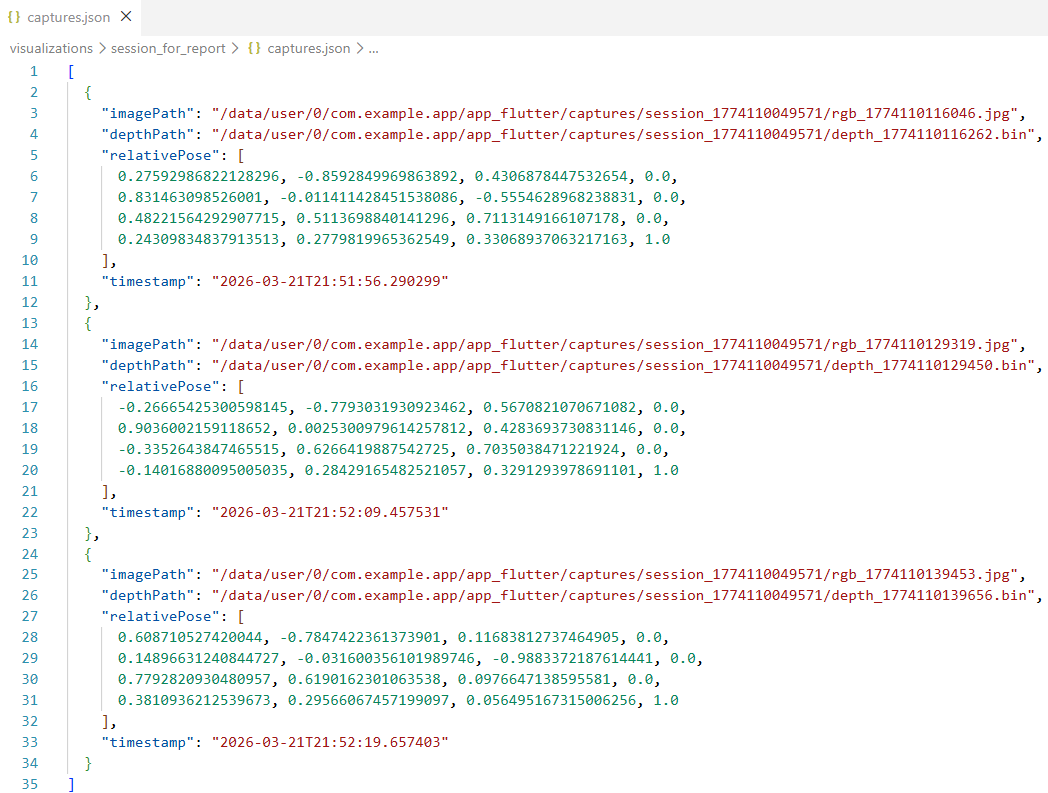
\includegraphics[width=1\textwidth]{Images/capture_data.png}}

    \vspace{20pt}

    \makebox[\textwidth][c]{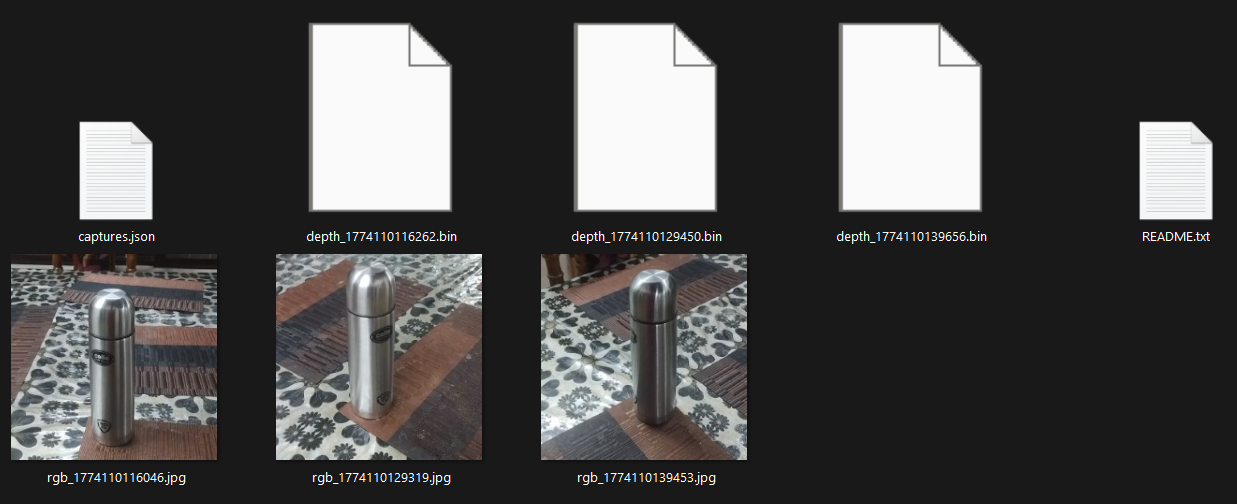
\includegraphics[width=1\textwidth]{Images/stored_session_data.png}}
    \vspace{10pt}
    \caption{Output data format illustrating the stored RGB image path, paired depth map, and the $4 \times 4$ camera pose matrix.}
    \label{fig:captured_data}
\end{figure}

\pagebreak

\section{Depth Estimation via TensorFlow Lite MiDaS}
Once the 1:1 RGB image is captured, it is processed locally using an on-device TensorFlow Lite (TFLite) interpreter running the MiDaS (Small) architecture.

\subsection{Image Processing and Inference}
The captured high-resolution square image is downscaled to a strict $256 \times 256$ pixel resolution, matching the input tensor shape expected by the MiDaS model. Pixel integers $(0\text{--}255)$ are converted into 32-bit floating-point arrays and normalized between $0.0$ and $1.0$ across the RGB channels.

The inference engine executes the model, which outputs an inverse relative depth map. A significant implementation hurdle was observed: the raw output yielded inverted depth (making distant objects appear erroneously close). This was resolved programmatically by applying an inverse scale mapping formula: $Z = 0.5 + (D_{norm} \times 2.5)$, where $D_{norm}$ is the normalized depth value. This effectively bounds the predicted spatial range between $0.5$ meters (foreground) and $3.0$ meters (background).

\begin{figure}[H]
    \centering
    \makebox[\textwidth][c]{%
        \begin{minipage}[t]{0.53\textwidth}
            \centering
            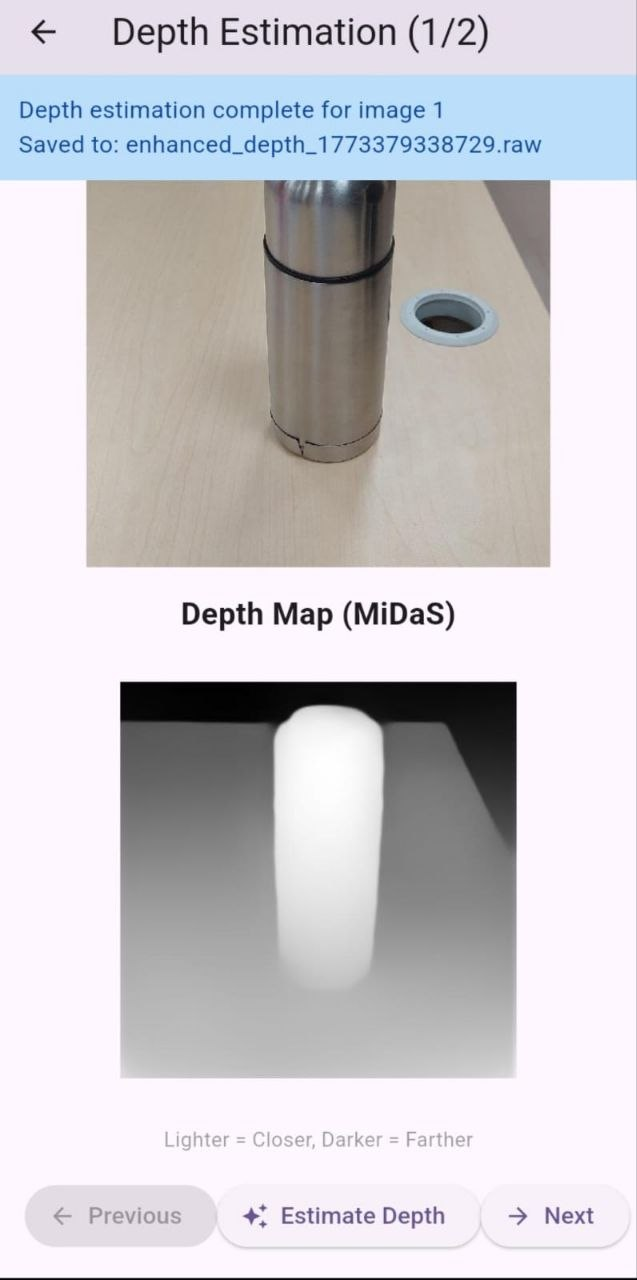
\includegraphics[width=\linewidth]{Images/Depth1.jpg}
        \end{minipage}\hspace{0.04\textwidth}%
        \begin{minipage}[t]{0.53\textwidth}
            \centering
            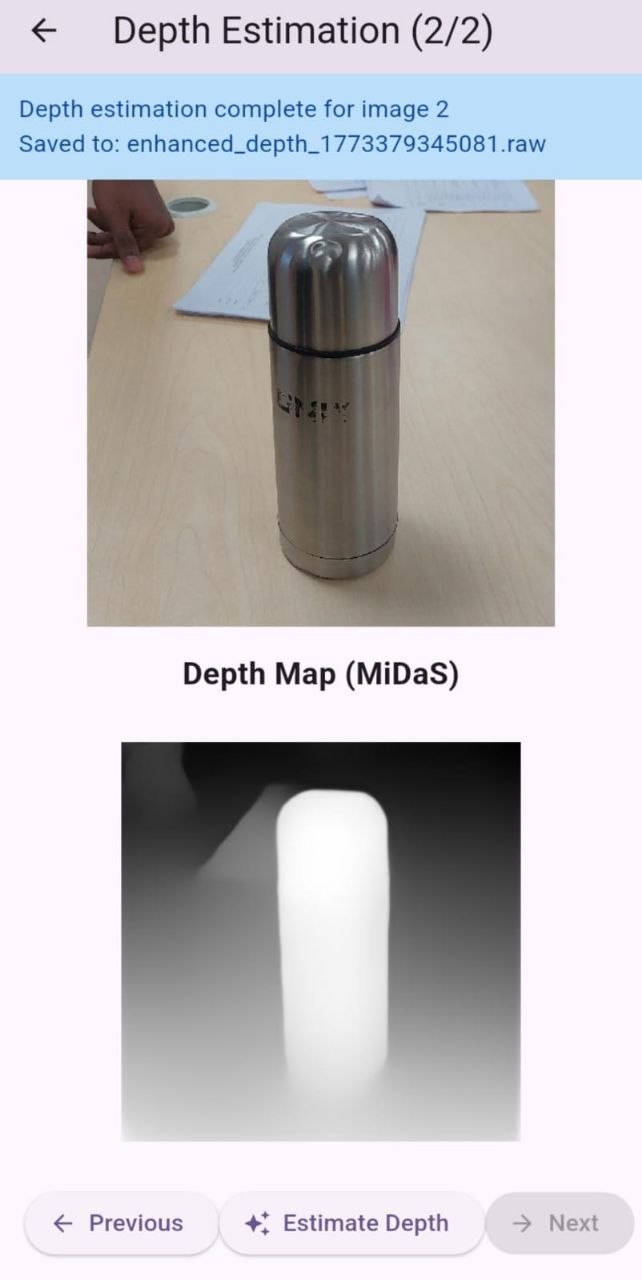
\includegraphics[width=\linewidth]{Images/Depth2.jpg}
        \end{minipage}%
    }
    \vspace{10pt}
    \caption{Application screenshot displaying the original captured RGB image (left) alongside its generated grayscale depth map (right).}
    \label{fig:depth_map_result}
\end{figure}
\pagebreak

\section{Point Cloud Generation}
The transformation from 2D arrays to a 3D coordinate space is achieved via intrinsic camera back-projection.

\subsection{Back-Projection Implementation}
Using a pinhole camera model, the algorithm iterates through every pixel $p(u, v)$ in the resultant depth map. Given the estimated depth $Z$ at that pixel, and the estimated horizontal/vertical focal lengths $(f_x, f_y)$ combined with the optical center $(c_x, c_y)$, the absolute 3D coordinates $(X, Y, Z)$ are reconstructed. Each coordinate is simultaneously mapped back to the original high-resolution RGB image to extract the exact $R, G, B$ color values, embedding the visual texture directly into the geometric points. Stride factors were implemented to allow dynamic downsampling, ensuring the mobile device's memory limits are not exceeded while maintaining dense environmental structures.

\begin{figure}[H]
    \centering
    \makebox[\textwidth][c]{%
        \begin{minipage}[t]{0.53\textwidth}
            \centering
            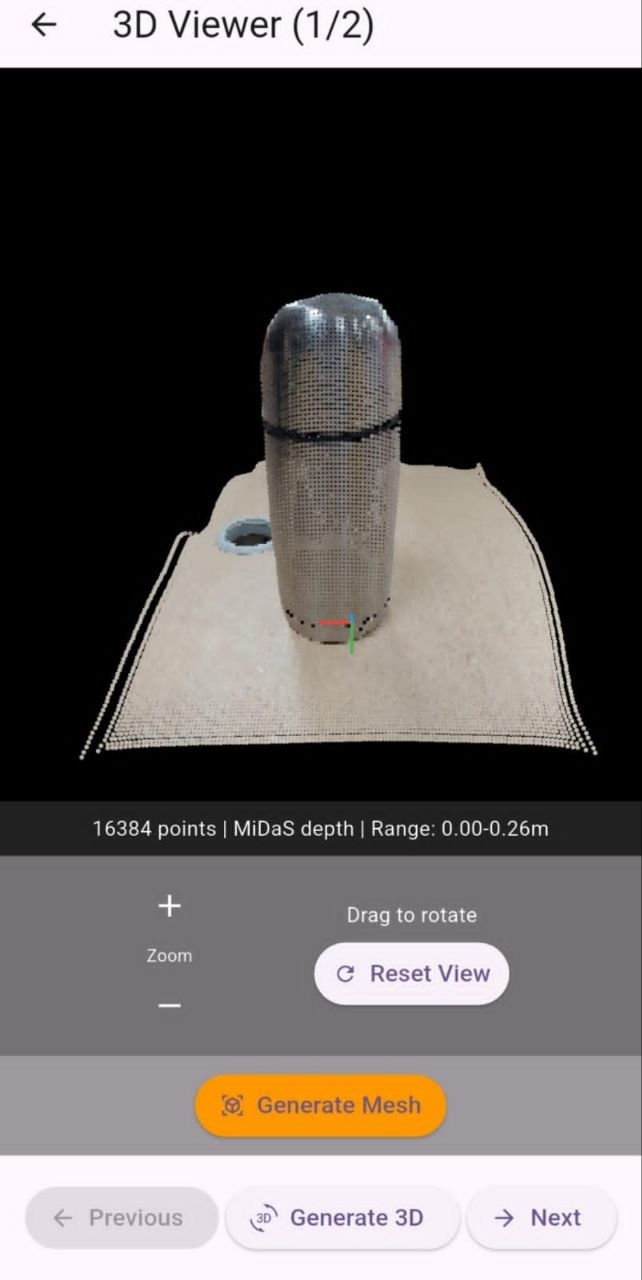
\includegraphics[width=\linewidth]{Images/Pointcloud1.jpg}
        \end{minipage}\hspace{0.04\textwidth}%
        \begin{minipage}[t]{0.53\textwidth}
            \centering
            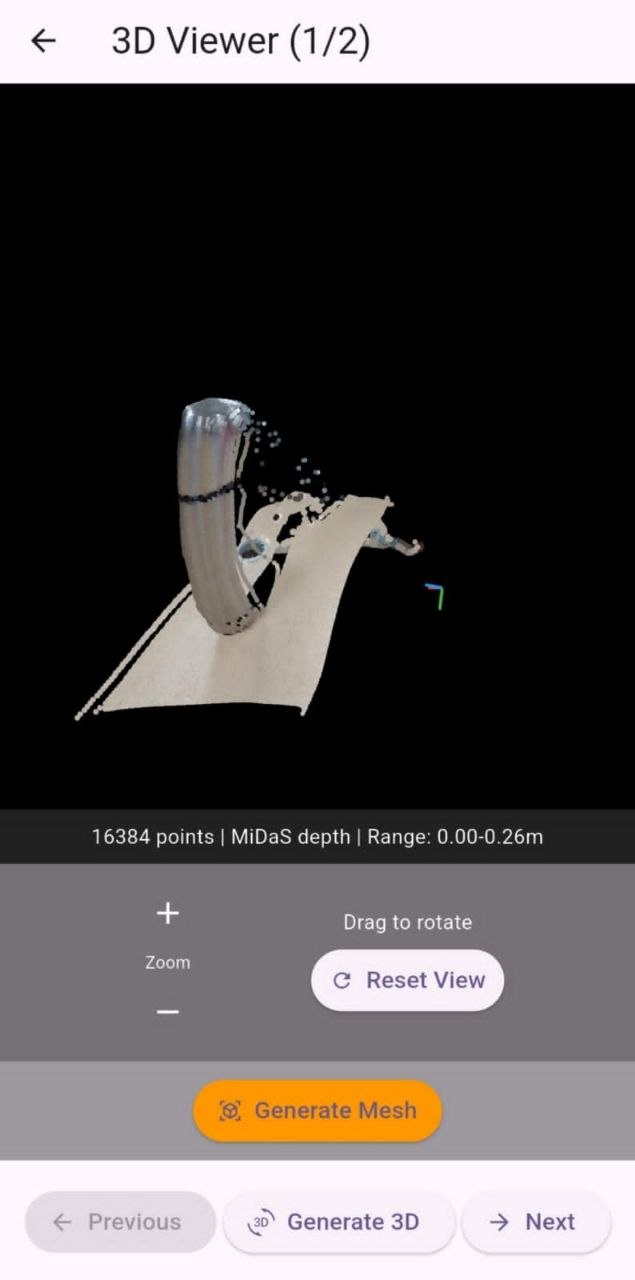
\includegraphics[width=\linewidth]{Images/Pointcloud2.jpg}
        \end{minipage}%
    }
    \vspace{10pt}
    \caption{Interactive 3D point cloud rendered within the mobile viewer, built from estimated depth data and mapped RGB colors.}
    \label{fig:point_cloud}
\end{figure}
\pagebreak

\section{Surface Reconstruction and Mesh Rendering}
The final phase involves deriving a continuous topological surface from the discrete point cloud, enabling the object's use in standard 3D rendering engines.

\subsection{The Rolling Ball Algorithm}
To create valid triangular faces connecting the points, the \textbf{Ball Pivoting Algorithm (Rolling Ball Algorithm)} was implemented.
The algorithm simulates a virtual ball of a defined radius (e.g., $r = 0.05$ units) resting on three points in the cloud, forming a seed triangle. The ball then rolls over the edge of this triangle until it catches a new adjacent point without encapsulating any other points inside its volume, thereby forming a new adjacent triangle.

To ensure the mesh is structurally sound and to prevent gaping holes across varying point densities, several heuristic constraints were added:
\begin{itemize}
    \item \textbf{Maximum Edge Length:} Triangles are rejected if the distance between vertices exceeds a threshold, preventing stretched, artificial geometry between completely separate objects (e.g., an object and the wall behind it).
    \item \textbf{Neighborhood Search Constraints:} Optimization was performed using a localized voxel grid, which drastically reduced computation time by testing the virtual ball only against nearby points rather than iterating over the entire cloud.
\end{itemize}

\subsection{Device Rendering and Asset Export}
\begin{sloppypar}
The generated mesh layout is rendered natively on the device using the \texttt{flutter\_cube} parsing library.
Vertex color shading is used to render the object through its assigned texture data, overriding artificial lighting shaders to preserve the original appearance.

Furthermore, an exporter module serializes these data structures into widely supported graphics formats.
The system exports a Wavefront \texttt{.obj} file containing geometric vertices (\texttt{v}) and polygonal faces (\texttt{f}).
For textures, it generates a matching Material Template Library (\texttt{.mtl}) file and a \texttt{.png} image.
The UV map is computed to align mesh triangles with their corresponding regions in the generated 2D texture, enabling cross-platform sharing and analysis in standard 3D software.
\end{sloppypar}

\begin{figure}[H]
    \centering
    \makebox[\textwidth][c]{%
        \begin{minipage}[t]{0.53\textwidth}
            \centering
            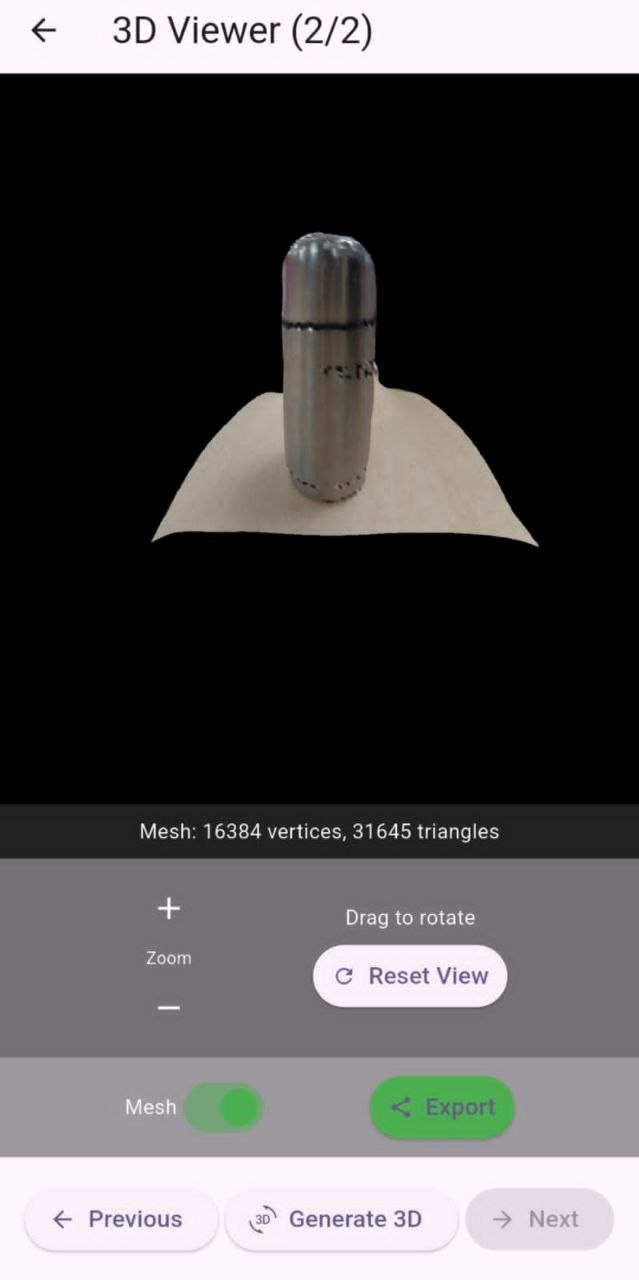
\includegraphics[width=\linewidth]{Images/Mesh1.jpg}
        \end{minipage}\hspace{0.04\textwidth}%
        \begin{minipage}[t]{0.53\textwidth}
            \centering
            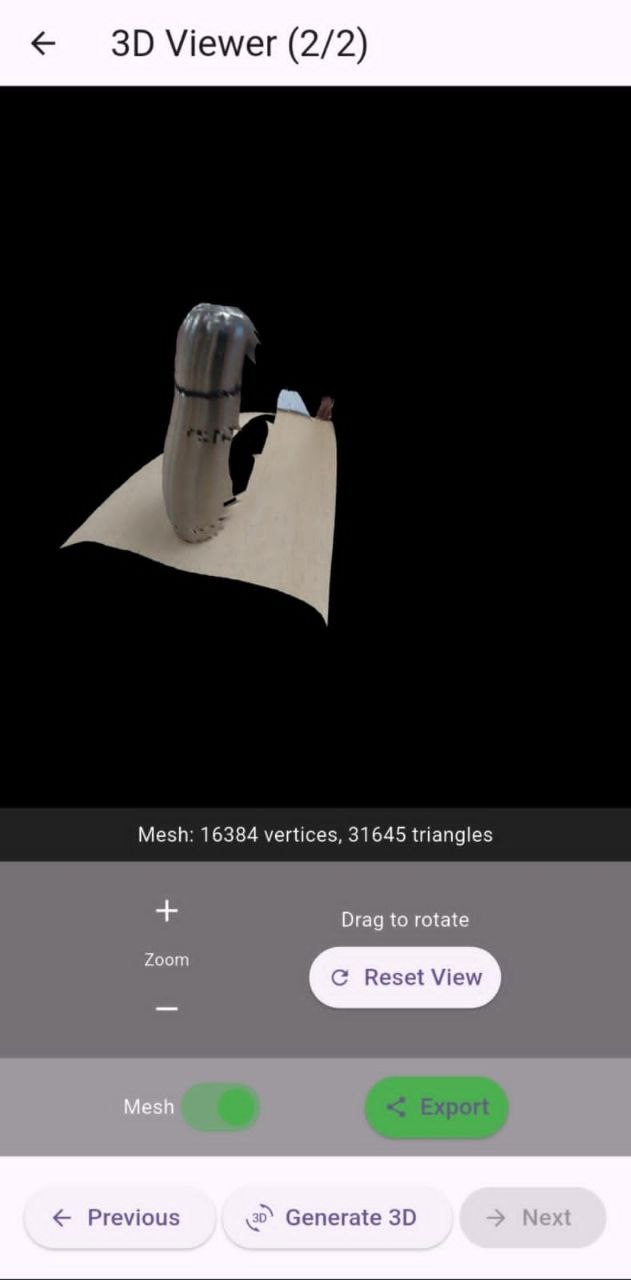
\includegraphics[width=\linewidth]{Images/Mesh2.jpg}
        \end{minipage}%
    }
    \vspace{10pt}
    \caption{The fully generated 3D mesh displayed within the mobile application's native rendering engine.}
    \label{fig:mesh_render}
\end{figure}

\begin{figure}[H]
    \centering
    \makebox[\textwidth][c]{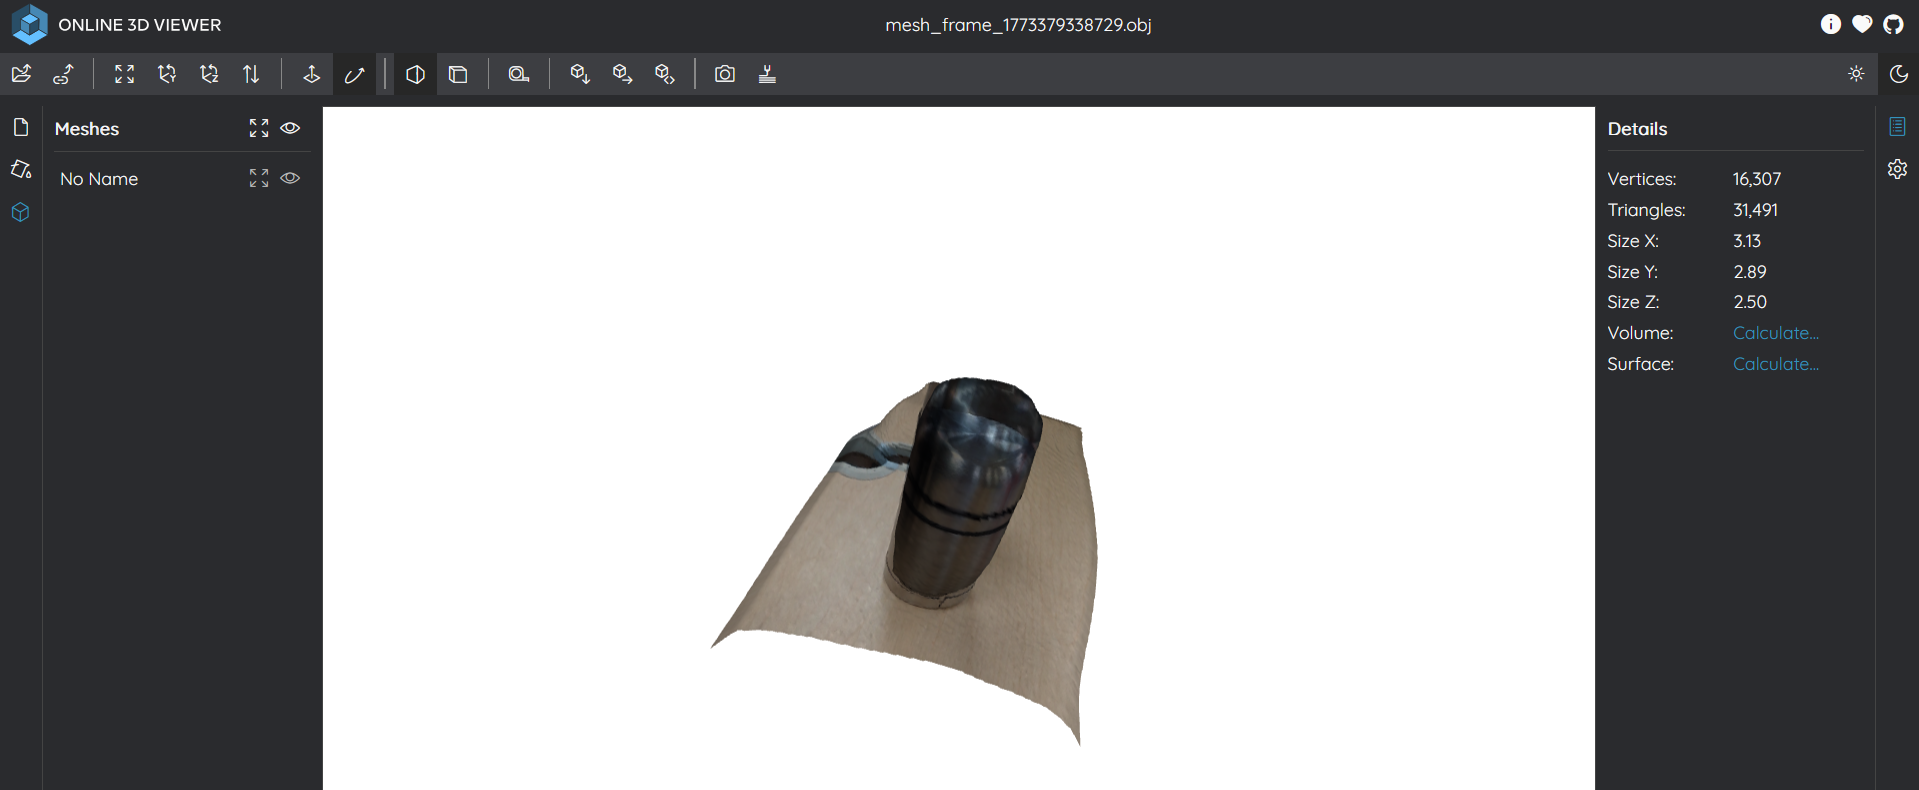
\includegraphics[width=1.25\textwidth]{Images/external1.png}}

    \vspace{16pt}

    \makebox[\textwidth][c]{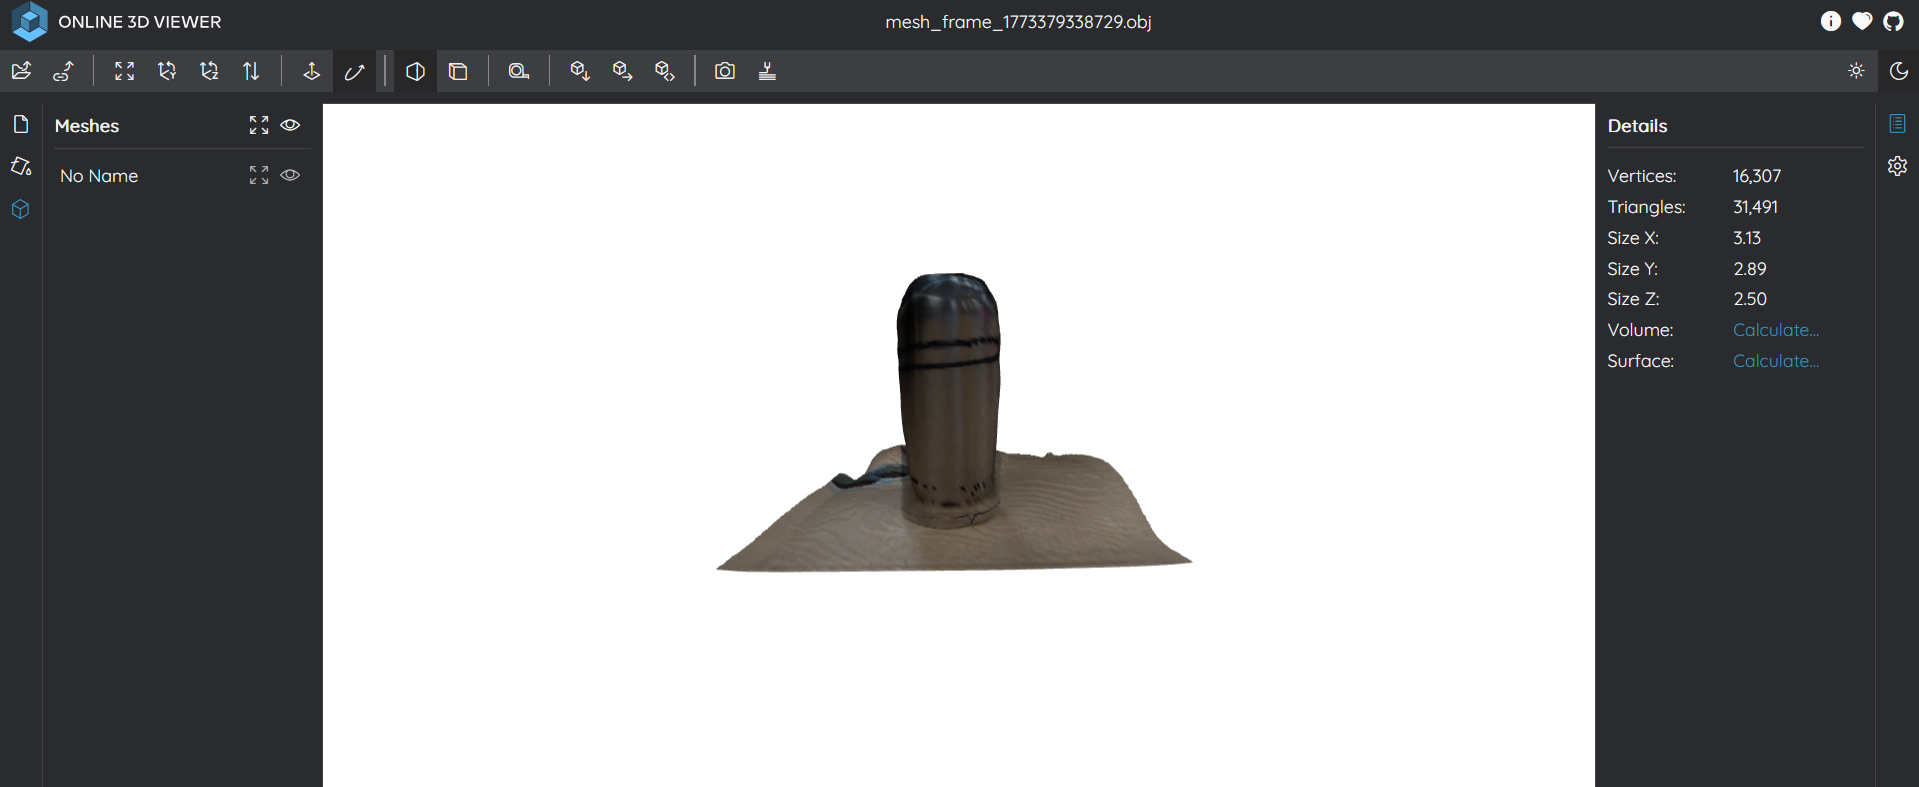
\includegraphics[width=1.25\textwidth]{Images/external2.png}}

    \vspace{10pt}
    \caption{The exported \texttt{.obj}, \texttt{.mtl}, and \texttt{.png} texture files loaded into a third-party 3D viewer, demonstrating cross-platform portability.}
    \label{fig:mesh_export}
\end{figure}